\documentclass[11pt,a4paper,spanish]{book}
\usepackage{unir}
\usepackage{tcolorbox}
\usepackage{float}
\usepackage{courier}
\usepackage{listings}
\lstset{basicstyle=\ttfamily\small, breaklines=true, frame=single, postbreak=\mbox{\textcolor{red}{$\hookrightarrow$}\space}}

%---------------------------
%título del trabajo y autor
%---------------------------
\title{ Algoritmos cuánticos para optimización de rutas}
\titulacion{ Máster en Computación Cuántica}
\author{ Gustavo Recalde Vásquez}
\date{ 19 de junio de 2024}
\director{ Francisco Costa Cano}
\nombreciudad{ Quito - Ecuador}

%---------------------------
%marges
%---------------------------
%\usepackage[margin=1.9cm]{geometry}
%---------------------------
%---------------------------
%---------------------------
%---------------------------
\begin{document}
\renewcommand{\listfigurename}{Índice de Ilustraciones}
\renewcommand{\listtablename}{Índice de Tablas}
\renewcommand{\contentsname}{Índice de Contenidos}
\renewcommand{\figurename}{Figura}
\renewcommand{\tablename}{Tabla} 

\maketitle
\frontmatter
\tableofcontents
\listoffigures
\listoftables

\chapter{Resumen}

Este trabajo aborda el desarrollo y aplicación de algoritmos cuánticos para la optimización de rutas de entrega y carga en la empresa Wolf. Mediante el empleo de técnicas de computación cuántica, se propone mejorar la eficiencia en la distribución y el uso del espacio de carga en una flota de camiones. La investigación incluye el diseño, simulación y evaluación de algoritmos cuánticos, comparándolos con métodos clásicos para demostrar su potencial superior. Los resultados indican que los algoritmos cuánticos pueden ofrecer soluciones más eficientes, impactando positivamente en la reducción de costos y tiempos de entrega.

{\bf Palabras Clave:} computación cuántica, optimización de rutas, logística, algoritmos cuánticos, simulación.


\chapter{Abstract}

This work addresses the development and application of quantum algorithms for the optimization of delivery routes and load management for Wolf Company. Using quantum computing techniques, it aims to enhance efficiency in distribution and optimize cargo space utilization across a fleet of trucks. The study involves designing, simulating, and evaluating quantum algorithms, comparing them with classical methods to demonstrate their superior potential. The results suggest that quantum algorithms can offer more efficient solutions, positively impacting cost reduction and delivery times.

{\bf Keywords:} quantum computing, route optimization, logistics, quantum algorithms, simulation.

\mainmatter
\chapter{Introducción}

Este trabajo se centra en el desarrollo y aplicación de algoritmos cuánticos para la optimización de rutas de entrega y volumen de carga en la empresa Wolf. Utilizando técnicas de computación cuántica, se busca abordar los desafíos específicos relacionados con la eficiencia en la distribución y el aprovechamiento del espacio de carga en una flota de camiones. 

%Típicamente una introducción tiene tres apartados:

\section{Motivación.}

    El transporte y la logística son vitales para la economía global, pero enfrentan problemas significativos relacionados con la optimización de rutas y la carga de vehículos. Las soluciones actuales son a menudo ineficientes, llevando a un uso subóptimo de recursos, aumento de costos y tiempo de entrega. Este trabajo identifica y aborda estas ineficiencias utilizando algoritmos cuánticos, que prometen una capacidad superior para manejar la complejidad y dinamismo de tales sistemas.
    La importancia de optimizar rutas de entrega y carga se magnifica en contextos de alta demanda y diversidad geográfica, como es el caso de las empresas de logística. Los desafíos incluyen la gestión eficiente de múltiples puntos de recolección y distribución, la variabilidad en el tamaño y volumen de los paquetes, y restricciones temporales estrictas. La computación cuántica ofrece un enfoque prometedor para superar estos retos, lo que podría resultar en una significativa reducción de costos operativos y mejora en la eficiencia del servicio.

\section{Planteamiento del trabajo.}

    Este estudio se centra en el desarrollo y evaluación de algoritmos cuánticos diseñados para optimizar las rutas de entrega y la carga de camiones para la empresa Wolf. Se analizarán y compararán estos algoritmos con métodos clásicos de optimización para determinar su viabilidad y eficacia. Dividiremos el problema en tres partes específicas:

    \begin{itemize}
    \item Optimización de rutas: Desarrollar un algoritmo que mejore la eficiencia de las rutas de entrega, teniendo en cuenta la ubicación geográfica de los puntos de distribución, el tamaño y volumen de los paquetes, y los intervalos de tiempo de entrega.
    
    \item Planificación de itinerarios: Crear un sistema que detalle el tiempo estimado de llegada para cada vehículo a todos los puntos de distribución.
    
    \item Optimización de la carga: Mejorar el proceso de carga de los vehículos, ordenando los paquetes de manera que se maximice el uso del espacio disponible y se optimice la eficiencia del transporte.
    
    La investigación evaluará la aplicabilidad de varios algoritmos cuánticos, incluyendo el quantum annealing y el algoritmo de Grover, y utilizará plataformas como IBM Quantum, D-Wave y Rigetti.
    \end{itemize}
    
\section{Estructura del trabajo.}

    Este trabajo estará organizado en los siguientes capítulos para abordar de manera sistemática el problema de investigación:

    \begin{itemize}
    \item \textbf{Introducción:} Presentación del problema, justificación y objetivos del estudio.
    Fundamentos Teóricos: Explicación de los conceptos básicos de la mecánica cuántica y la computación cuántica necesarios para entender los algoritmos utilizados.
	
	\item \textbf{Contexto y Estado de la Técnica:} Revisión de la literatura existente sobre logística, optimización de rutas, y el impacto de la computación cuántica en estos campos. Discusión sobre los métodos clásicos y cuánticos, y las tendencias actuales en la investigación cuántica aplicada a la logística.
	
	\item \textbf{Objetivos:} Definición del objetivo general y los objetivos específicos del estudio, incluyendo las métricas de éxito y los resultados esperados.
	
	\item \textbf{Identificación de Requisitos:} Análisis detallado de los requisitos técnicos, operativos y de negocio que los algoritmos cuánticos deben satisfacer para abordar efectivamente los desafíos de optimización en la empresa Wolf.
	
	\item \textbf{Fundamentos Teóricos:} Explicación de los conceptos básicos de optimización, mecánica cuántica y la computación cuántica necesarios para entender los algoritmos utilizados tanto clásicos como cuánticos, incluyendo qubits, superposición, entrelazamiento, interferencia cuántica, puertas cuánticas, y circuitos cuánticos.
	
	\item \textbf{Desarrollo de la solución:} Descripción de las técnicas y herramientas seleccionadas para el desarrollo de los algoritmos cuánticos, así como la metodología de comparación con sistemas clásicos. Incluye el diseño y codificación de los algoritmos cuánticos, seguido de la realización de simulaciones computacionales para evaluar su rendimiento. Este capítulo abarca la generación de la muestra de clientes, la implementación de algoritmos clásicos y genéticos, y la implementación de algoritmos cuánticos como Quantum Annealing (QA) y Quantum Approximate Optimization Algorithm (QAOA). Se detalla cada paso en el desarrollo de la solución y los códigos fuente utilizados en la implementación.
		
	\item \textbf{Resultados y Análisis:} Presentación y análisis de los resultados obtenidos, comparando las soluciones cuánticas con las clásicas y genéticas. Evaluación de la eficiencia y eficacia de los algoritmos cuánticos en términos de mejora de rutas y costos operativos.
	
	\item \textbf{Conclusiones y Recomendaciones:} Síntesis de los hallazgos clave del estudio, recomendaciones para futuras investigaciones y aplicaciones prácticas, y una reflexión sobre el impacto potencial de la computación cuántica en la logística y la gestión de la cadena de suministro.
	
\end{itemize}

\chapter{Contexto y Estado de la Técnica}

La logística y la optimización de rutas han sido áreas de estudio intensivo debido a su impacto crítico en la economía y la sostenibilidad ambiental. Con el avance de la tecnología, los métodos para abordar estos problemas han evolucionado significativamente. Desde los enfoques heurísticos clásicos hasta los algoritmos de optimización avanzados, el campo ha visto una considerable transformación. La introducción de la computación cuántica ha abierto nuevas avenidas de investigación, prometiendo superar las limitaciones de los algoritmos clásicos al manejar problemas de optimización NP-difíciles con una eficiencia potencialmente mayor \citep{nielsenChuang}.

El desarrollo de algoritmos cuánticos específicos para la optimización, como quantum annealing, QAOA y paseo cuántico, ha mostrado ser prometedor en la simulación de escenarios complejos dentro de la optimización de rutas . Estos algoritmos han sido aplicados en diversos contextos, demostrando la capacidad de la computación cuántica para explorar eficientemente grandes espacios de soluciones \citep{QWalk-Based}.

\section{Aplicación de la Computación Cuántica en Transporte y Logística}

En el contexto del transporte y la logística, los algoritmos de paseo cuántico, por ejemplo, han sido propuestos como una metodología efectiva para optimizar redes de transporte \citep{quantumTransportOpt}. Este enfoque sugiere una mejora significativa en la planificación de rutas, permitiendo no solo la reducción de costos y tiempos de operación sino también la mejora en la sostenibilidad de las operaciones logísticas.

La investigación previa en algoritmos de routing clásicos también ha proporcionado un sólido fundamento para los desarrollos cuánticos, demostrando la importancia de robustecer los algoritmos frente a la incertidumbre y la variabilidad en las demandas y condiciones operativas \citep{transportationScience}. Esta base teórica es crucial para entender las áreas donde la computación cuántica puede ofrecer las mejoras más significativas.

\section{Tendencias Actuales y Financiación en la Investigación Cuántica}

Con el incremento del interés y la inversión en tecnologías cuánticas, ha habido un notable 'auge cuántico' con financiación privada y gubernamental fluyendo hacia startups y proyectos de investigación cuántica \citep{quantumTech}. Plataformas como IBM Quantum, D-Wave y Rigetti han sido líderes en proporcionar acceso a tecnologías cuánticas, lo que ha facilitado el desarrollo y la prueba de algoritmos cuánticos en un contexto real \citep{qiskit, dwaveOcean}.

\chapter{Objetivos}

\section{Objetivo General}
Mejorar significativamente la eficiencia de las rutas de entrega y carga de la flota de camiones de la empresa Wolf a través del desarrollo y la implementación de algoritmos cuánticos.

\section{Objetivos Específicos}

\begin{itemize}
    \item Desarrollar un algoritmo cuántico para la optimización de rutas de entrega que considere variables clave como la geolocalización de los puntos de entrega. Este algoritmo debe demostrar una mejora del 10\% en la eficiencia de las rutas comparado con los métodos de optimización clásicos utilizados actualmente por la empresa. Esta métrica ha sido definida por la institución que proporciona los datos en base a metas internas.

    \item Implementar un sistema de planificación de itinerarios detallados utilizando el algoritmo cuántico desarrollado para predecir con precisión el tiempo estimado de llegada de cada camión en todos los puntos de distribución.

    \item Optimizar el proceso de carga de los vehículos para maximizar el uso del espacio disponible y mejorar la eficiencia en el transporte, logrando una reducción de al menos el 5\% en el número de viajes necesarios por la misma cantidad de cargas comparado con el sistema actual, porcentaje esperado de acuerdo a las metas definidas internamente en la empresa.

    \item Evaluar la viabilidad técnica y económica de la implementación de soluciones cuánticas en la logística de transporte, incluyendo un análisis de costos y beneficios que identifique los ahorros potenciales en costos operativos y tiempos de entrega.

    \item Documentar y difundir los resultados y metodologías del proyecto a través de publicaciones en revistas científicas y presentaciones en conferencias relevantes en el campo de la computación cuántica y la logística, para compartir conocimientos y prácticas con la comunidad académica y profesional.

\end{itemize}

\section{Metodología de Trabajo}

Para alcanzar estos objetivos, se seguirán una serie de pasos metodológicos estructurados:

\begin{itemize}

    \item Revisión de literatura: Estudio exhaustivo de trabajos previos en computación cuántica aplicada a la optimización y algoritmos clásicos de optimización de rutas.

    \item Desarrollo de algoritmos: Diseño y codificación de algoritmos cuánticos basados en las necesidades identificadas.

    \item Simulaciones y pruebas: Realización de simulaciones computacionales para validar la eficacia de los algoritmos cuánticos desarrollados.

    \item Análisis comparativo: Comparación de los nuevos algoritmos con los sistemas tradicionales para evaluar las mejoras en eficiencia y costos.

    \item Evaluación y ajustes: Iteraciones basadas en los resultados de las pruebas para perfeccionar los algoritmos y sistemas implementados.

    \item Documentación y publicación: Preparación de documentos que describan el proceso y los resultados obtenidos para su revisión y publicación.

\end{itemize}

\chapter{Identificación de Requisitos}

Para abordar efectivamente los desafíos de optimización de rutas y carga, es esencial identificar y analizar minuciosamente los requisitos específicos que los algoritmos cuánticos deben satisfacer. Esta sección detalla los criterios técnicos, operativos y de negocio que han sido considerados para la formulación de la solución cuántica propuesta. Los requisitos se han dividido en tres categorías principales: técnicos, operativos y de negocio.


\section{Requisitos Técnicos}

\begin{itemize}
	\item \textbf{Capacidad de Escalabilidad:} El algoritmo debe ser escalable para manejar incrementos en el número de vehículos y destinos sin degradar significativamente su rendimiento.
	\item \textbf{Precisión en la Optimización:} Alta precisión en la determinación de rutas óptimas y asignaciones de carga, para asegurar la máxima eficiencia posible.
	\item \textbf{Rapidez de Procesamiento:} Capacidad para generar soluciones en un tiempo competitivo, especialmente importante durante los periodos de alta demanda.
	\item \textbf{Integración con Sistemas Existentes:} Facilidad de integración con los sistemas de gestión logística ya implementados en Wolf.
	\item \textbf{Adaptabilidad a Condiciones Variables:} Flexibilidad para ajustarse a cambios imprevistos en rutas o prioridades de entrega.
\end{itemize}

\section{Requisitos Operativos}

\begin{itemize}
	\item \textbf{Interfaz de Usuario Amigable:} Interfaces claras y accesibles para que los operadores logísticos puedan utilizar el sistema sin necesidad de conocimientos técnicos avanzados.
	\item \textbf{Capacitación de Personal:} Tutorial de formación para los empleados en el manejo de la plataforma que se usara para el manejo del algoritmo desarrollado.
\end{itemize}

\section{Requisitos de Negocio}

\begin{itemize}
	\item \textbf{Costo-Efectividad:} La solución debe justificar la inversión inicial y los costos operativos mediante ahorros tangibles en eficiencia y tiempo empleados y definidos en los objetivos.
	\item \textbf{Mejora en la Satisfacción del Cliente:} Contribuir a una mayor puntualidad y precisión en las entregas, mejorando la satisfacción del cliente.

\end{itemize}

\chapter{Fundamentos Teóricos}

\section{Introducción a los Problemas de Optimización}

La optimización es fundamental en la logística y la gestión de la cadena de suministro, enfocándose en mejorar la eficiencia, reducir costos y optimizar el rendimiento general. Diversos problemas de optimización en este campo han sido abordados tradicionalmente mediante técnicas de computación clásica. Sin embargo, con el avance de la computación cuántica, estos problemas han adoptado nuevos enfoques que explotan las propiedades únicas de la mecánica cuántica. Por lo tanto, se han dividido en dos grupos para su análisis detallado: optimización clásica y optimización cuántica.

\section{Optimización Clásica}

\subsection{Problemas de Ruteo de Vehículos (VRP):} 
	
	El problema de ruteo de vehículos (VRP) implica la planificación eficiente de rutas para una flota de vehículos que deben entregar productos a varios destinos. El objetivo principal es minimizar la distancia total recorrida o el costo total del transporte, mientras se satisfacen ciertas restricciones como la capacidad de los vehículos y las ventanas de tiempo para las entregas.
	
	\textbf{Algoritmos Clásicos Aplicables:}
	\begin{itemize}
		\item \textbf{Algoritmo de Clarke-Wright (CW):} Es un método heurístico basado en el concepto de ahorro de costos, combinando rutas individuales en una sola ruta para minimizar la distancia recorrida \cite{clarkeWright}.
		\item \textbf{Algoritmo de Búsqueda Tabú:} Utiliza una lista tabú para evitar ciclos y explorar soluciones alternativas mediante búsquedas locales iterativas \cite{glover1989tabu}.
		\item \textbf{Algoritmo de Colonia de Hormigas (ACO):} Se inspira en el comportamiento de las hormigas para encontrar rutas óptimas, utilizando feromonas para guiar la búsqueda hacia soluciones eficientes \cite{dorigo1997ant}.
		\item \textbf{Optimización por Enjambre de Partículas (PSO):} Emplea partículas que exploran el espacio de soluciones de manera colaborativa, ajustando sus posiciones en base a su experiencia y la de sus vecinas \cite{kennedy1995particle}.
        \item \textbf{Algoritmo 2-opt:} El algoritmo 2-opt es una técnica de optimización local utilizada para mejorar soluciones de problemas de optimización combinatoria, como el (TSP). Este algoritmo funciona mediante la eliminación de dos aristas de un tour y la reconexión de las subrutas resultantes de la manera más óptima. Repite este proceso iterativamente hasta que no se pueden encontrar más mejoras. La simplicidad y eficacia del 2-opt lo convierten en una herramienta valiosa para refinar soluciones generadas por otros algoritmos heurísticos. \cite{lawler1985}

	\end{itemize}
	
\subsection{Problemas de Diseño de Redes Logísticas:} 
	
	El diseño de redes logísticas incluye la ubicación óptima de instalaciones como almacenes y centros de distribución, así como el diseño de las rutas de transporte entre estas instalaciones y los clientes. El objetivo es minimizar los costos de transporte, almacenamiento y manejo, garantizando al mismo tiempo un nivel adecuado de servicio al cliente.
	
	\textbf{Algoritmos Clásicos Aplicables:}
	\begin{itemize}
		\item \textbf{Programación Lineal Entera Mixta (MILP):} Utiliza técnicas de optimización matemática para resolver problemas de diseño de redes considerando restricciones y objetivos específicos \cite{nemhauser1999integer}.
		\item \textbf{Algoritmo de Recocido Simulado (SA):} Emula el proceso de enfriamiento de materiales para encontrar soluciones cercanas al óptimo global mediante la exploración del espacio de soluciones \cite{kirkpatrick1983optimization}.
		\item \textbf{Algoritmo de Búsqueda de Vecindad Variable (VNS):} Emplea una serie de búsquedas locales en diferentes vecindades para escapar de óptimos locales y encontrar mejores soluciones globales \cite{mladenovic1997variable}.
		\item \textbf{Algoritmo Genético (GA):} Utiliza técnicas de selección, cruce y mutación inspiradas en la evolución natural para explorar y explotar el espacio de soluciones \cite{holland1992adaptation}.
        \item \textbf{Algoritmo Greedy:}  selecciona iterativamente la próxima ciudad más cercana no visitada hasta que todas las ciudades han sido visitadas. Aunque no garantiza la solución óptima global, es fácil de implementar y proporciona soluciones razonablemente buenas en un tiempo de ejecución relativamente corto. \cite{Cormen2009}

  
	\end{itemize}
	
\subsection{Problemas de Carga de Contenedores:} 
	
	Los problemas de carga de contenedores se enfocan en maximizar la utilización del espacio dentro de los vehículos o contenedores, minimizando el número de viajes necesarios o el tiempo de carga y descarga. Es crucial optimizar cómo se apilan y organizan los objetos de diferentes tamaños y formas dentro de un espacio limitado.
	
	\textbf{Algoritmos Clásicos Aplicables:}
	\begin{itemize}
		\item \textbf{Algoritmo de Backtracking:} Explora todas las posibles combinaciones de colocación de objetos y retrocede cuando se encuentra una configuración no viable \cite{lawler1985knapsack}.
		\item \textbf{Algoritmo de Ramificación y Poda (B\&B):} Divide el problema en subproblemas más pequeños, descartando aquellos que no pueden llevar a una solución óptima \cite{lawler1966branch}.
		\item \textbf{Heurísticas de Envoltura:} Aplican reglas simples como el llenado de capas o niveles para organizar objetos dentro de contenedores \cite{coffman1978application}.
		\item \textbf{Algoritmo de Programación Dinámica (DP):} Descompone el problema en etapas más pequeñas, resolviendo cada una de manera óptima y construyendo una solución global \cite{bellman1966dynamic}.
	\end{itemize}
	
\subsection{Problemas de Programación:} 
	
	Los problemas de programación incluyen la optimización de horarios para la producción, el personal y el uso de máquinas, con el objetivo de minimizar los tiempos de espera y maximizar la eficiencia operativa. Esto es crucial para asegurar que los recursos sean utilizados de manera efectiva y que las operaciones se realicen de manera fluida.
	
	\textbf{Algoritmos Clásicos Aplicables:}
	\begin{itemize}
		\item \textbf{Método de Johnson:} Una técnica específica para problemas de secuenciación de dos máquinas que minimiza el tiempo total de procesamiento \cite{johnson1954optimal}.
		\item \textbf{Método de Programación por Restricciones (CP):} Utiliza restricciones lógicas y matemáticas para reducir el espacio de búsqueda y encontrar soluciones factibles y óptimas \cite{rossi2006handbook}.
		\item \textbf{Algoritmo de Cosegador Mínimo (MST):} Se aplica a problemas de programación de tareas en máquinas paralelas para minimizar el tiempo total de procesamiento \cite{graham1966bounds}.
		\item \textbf{Algoritmo de Branch and Bound (B\&B):} Descompone el problema en subproblemas y utiliza podas para eliminar subproblemas que no pueden contener la solución óptima \cite{lawler1966branch}.
	\end{itemize}


\section{Optimización Cuántica}

Con la llegada de la computación cuántica, han surgido nuevas técnicas que prometen abordar estos problemas de optimización de manera más eficiente. Entre las más destacadas se encuentran:

\begin{itemize}
	\item \textbf{Quantum Annealing (QA):} Un método de optimización que utiliza fluctuaciones cuánticas para encontrar el mínimo global de una función de costo. Es particularmente efectivo para resolver problemas de optimización combinatoria, como el VRP y la carga de contenedores \cite{phillipson2024}.
	\item \textbf{Quantum Approximate Optimization Algorithm (QAOA):} Un algoritmo híbrido que combina computación cuántica y clásica para aproximar soluciones a problemas de optimización. Ha mostrado ser prometedor en la optimización de rutas y otros problemas logísticos \cite{farhiQuantum}.
    \item \textbf{Quantum Walks Algorithm (QW):} Los paseos cuantciso son una generalización cuántica de los paseos aleatorios clásicos, donde la probabilidad de transición entre estados se reemplaza por amplitudes de probabilidad. Estos paseos cuánticos han mostrado ventajas significativas en la búsqueda y optimización de grafos, proporcionando una mayor velocidad y eficiencia en la exploración de grandes espacios de soluciones. Por ejemplo en el contexto del problema del viajante de comercio (TSP), los paseos cuánticos permiten una exploración más rápida y eficiente de las rutas posibles, mejorando la probabilidad de encontrar soluciones óptimas. \cite{kempe2003}
 
\end{itemize}

Para abordar estos algoritmos primero veremos un breve resumen de la Teoría Básica de Computación Cuántica.


\section{Teoría Básica de Computación Cuántica}

La computación cuántica aprovecha los principios de la mecánica cuántica para realizar cálculos de manera significativamente más eficiente que las computadoras clásicas para ciertos tipos de problemas. Los conceptos clave incluyen:

\subsection{Qubits y Superposición}

El qubit es la unidad fundamental de información en la computación cuántica. A diferencia de los bits clásicos, que pueden estar en uno de dos estados (0 o 1), un qubit puede estar en una superposición de ambos estados. Matemáticamente, un qubit se representa como:

\[ \lvert \psi \rangle = \alpha \lvert 0 \rangle + \beta \lvert 1 \rangle \]

donde \(\alpha\) y \(\beta\) son números complejos tales que \(|\alpha|^2 + |\beta|^2 = 1\). Este estado de superposición permite que un qubit almacene más información que un bit clásico \cite{nielsenChuang}.

\subsection{Entrelazamiento (Entanglement)}

El entrelazamiento es un fenómeno cuántico en el que los estados de dos o más qubits se correlacionan de tal manera que el estado de uno no puede describirse independientemente del estado del otro. Este fenómeno es esencial para muchos algoritmos cuánticos, ya que permite el procesamiento de información de manera altamente eficiente \cite{nielsenChuang}.

\subsection{Interferencia Cuántica}

La interferencia cuántica se refiere a la forma en que las probabilidades de diferentes caminos cuánticos se combinan. Los algoritmos cuánticos utilizan la interferencia para cancelar las amplitudes de probabilidad de los caminos no deseados y aumentar las de los caminos deseados. Esto es fundamental para el funcionamiento de muchos algoritmos cuánticos, como el algoritmo de Grover. \cite{groverAlgorithm}.

\subsection{Puertas Cuánticas}

Las puertas cuánticas son los bloques básicos de construcción de los circuitos cuánticos, análogos a las puertas lógicas en la computación clásica. Operan sobre qubits y pueden cambiar sus estados de una manera que aprovecha las propiedades cuánticas como la superposición y el entrelazamiento. A continuación, se describen algunas de las puertas cuánticas fundamentales, organizadas en orden de complejidad:

\begin{itemize}
	\item \textbf{Puerta Pauli-X (X):} Equivalente a una puerta NOT clásica, cambia el estado de un qubit de \(\lvert 0 \rangle\) a \(\lvert 1 \rangle\) y viceversa.
	\[
	X = \begin{pmatrix}
		0 & 1 \\
		1 & 0
	\end{pmatrix}
	\]
	
	\item \textbf{Puerta Pauli-Y (Y):} Introduce una rotación en el plano \(XY\) de la esfera de Bloch.
	\[
	Y = \begin{pmatrix}
		0 & -i \\
		i & 0
	\end{pmatrix}
	\]
	
	\item \textbf{Puerta Pauli-Z (Z):} Introduce una fase de \(\pi\) al estado \(\lvert 1 \rangle\).
	\[
	Z = \begin{pmatrix}
		1 & 0 \\
		0 & -1
	\end{pmatrix}
	\]
	
	\item \textbf{Puerta Hadamard (H):} Crea una superposición de estados. La operación de una puerta Hadamard sobre un qubit inicializado en \(\lvert 0 \rangle\) resulta en:
	\[
	H = \frac{1}{\sqrt{2}} \begin{pmatrix}
		1 & 1 \\
		1 & -1
	\end{pmatrix}
	\]
	\[ H \lvert 0 \rangle = \frac{1}{\sqrt{2}} (\lvert 0 \rangle + \lvert 1 \rangle) \]
	\[ H \lvert 1 \rangle = \frac{1}{\sqrt{2}} (\lvert 0 \rangle - \lvert 1 \rangle) \]
	
	\item \textbf{Puerta Phase (S):} Introduce una fase de \(\pi/2\) al estado \(\lvert 1 \rangle\). La puerta Phase se representa como:
	\[
	S = \begin{pmatrix}
		1 & 0 \\
		0 & i
	\end{pmatrix}
	\]
	Actúa sobre un qubit de la siguiente manera:
	\[ S \lvert 0 \rangle = \lvert 0 \rangle \]
	\[ S \lvert 1 \rangle = i \lvert 1 \rangle \]
	
	\item \textbf{Puerta T:} Introduce una fase de \(\pi/4\) al estado \(\lvert 1 \rangle\). La puerta T se representa como:
	\[
	T = \begin{pmatrix}
		1 & 0 \\
		0 & e^{i\pi/4}
	\end{pmatrix}
	\]
	Actúa sobre un qubit de la siguiente manera:
	\[ T \lvert 0 \rangle = \lvert 0 \rangle \]
	\[ T \lvert 1 \rangle = e^{i\pi/4} \lvert 1 \rangle \]
	
	\item \textbf{Puerta CNOT (Control-NOT):} Es una puerta de dos qubits donde el segundo qubit (qubit objetivo) es invertido si el primer qubit (qubit de control) está en el estado \(\lvert 1 \rangle\). Matemáticamente, la puerta CNOT se representa como:
	\[
	CNOT = \begin{pmatrix}
		1 & 0 & 0 & 0 \\
		0 & 1 & 0 & 0 \\
		0 & 0 & 0 & 1 \\
		0 & 0 & 1 & 0
	\end{pmatrix}
	\]
	Actúa sobre el estado de dos qubits.
	
	\item \textbf{Puerta Toffoli:} También conocida como la puerta CCNOT (Control-Control-NOT), es una puerta de tres qubits donde el tercer qubit (qubit objetivo) es invertido solo si los primeros dos qubits (qubits de control) están en el estado \(\lvert 1 \rangle\). Matemáticamente, la puerta Toffoli se representa como:
	\[
	Toffoli = \begin{pmatrix}
		1 & 0 & 0 & 0 & 0 & 0 & 0 & 0 \\
		0 & 1 & 0 & 0 & 0 & 0 & 0 & 0 \\
		0 & 0 & 1 & 0 & 0 & 0 & 0 & 0 \\
		0 & 0 & 0 & 1 & 0 & 0 & 0 & 0 \\
		0 & 0 & 0 & 0 & 1 & 0 & 0 & 0 \\
		0 & 0 & 0 & 0 & 0 & 1 & 0 & 0 \\
		0 & 0 & 0 & 0 & 0 & 0 & 0 & 1 \\
		0 & 0 & 0 & 0 & 0 & 0 & 1 & 0
	\end{pmatrix}
	\]
	Actúa sobre el estado de tres qubits.
	
\end{itemize}

\subsection{Circuitos Cuánticos}

Un circuito cuántico es una secuencia de puertas cuánticas aplicadas a uno o más qubits. Estos circuitos son utilizados para implementar algoritmos cuánticos. Un circuito típico incluye la preparación del estado inicial, la aplicación de una serie de puertas cuánticas y la medición del estado final de los qubits \cite{nielsenChuang}.

\subsection{Algoritmos Cuánticos}

Los algoritmos cuánticos aprovechan las propiedades cuánticas para resolver problemas de manera más eficiente que los algoritmos clásicos. Algunos de los algoritmos cuánticos más destacados incluyen:

\begin{itemize}
	\item \textbf{Algoritmo de Shor:} Factoriza números enteros en tiempo polinomial, resolviendo el problema de factorización de manera mucho más rápida que los mejores algoritmos clásicos conocidos \cite{shorAlgorithm}.
	\item \textbf{Algoritmo de Grover:} Proporciona una aceleración cuadrática para la búsqueda en bases de datos no ordenadas \cite{groverAlgorithm}.
	\item \textbf{Quantum Annealing:} Utiliza fluctuaciones cuánticas para resolver problemas de optimización combinatoria \cite{farhiQuantum}.
\end{itemize}

Estos algoritmos han mostrado una ventaja significativa en ciertos tipos de problemas, aunque su implementación práctica aún está en desarrollo \cite{nielsenChuang}.

\subsection{Hardware de Computación Cuántica}

Los dispositivos de computación cuántica actuales utilizan diferentes tecnologías para implementar qubits, incluyendo:

\begin{itemize}
	\item \textbf{Iones atrapados:} Utilizan iones individuales atrapados y manipulados con láseres.
	\item \textbf{Superconductores:} Utilizan circuitos superconductores para crear qubits a bajas temperaturas.
	\item \textbf{Puntos cuánticos:} Utilizan semiconductores para confinar electrones y crear qubits.
\end{itemize}

Cada tecnología tiene sus propias ventajas y desafíos, y la investigación continúa para desarrollar dispositivos cuánticos más robustos y escalables \cite{gibneyQuantumTech}.

\section{Desarrollo de Algoritmos Cuánticos}

\subsection{Quantum Annealing}

Quantum Annealing (QA) es una técnica de optimización cuántica que aprovecha los principios de la mecánica cuántica para encontrar soluciones óptimas a problemas de optimización combinatoria. Este método es especialmente efectivo para problemas NP-difíciles, como el problema de ruteo de vehículos (VRP) y la carga de contenedores.

\subsubsection{Principios de Quantum Annealing}

El QA se basa en el modelo de Computación Adiabática Cuántica (AQC). La idea central es preparar el sistema cuántico en el estado fundamental de un Hamiltoniano inicial sencillo, \(H_0\). Luego, el sistema evoluciona adiabáticamente hacia un Hamiltoniano final \(H_1\), cuyo estado fundamental codifica la solución del problema de optimización. La evolución se describe mediante el Hamiltoniano dependiente del tiempo \(H(t)\):

\[ H(t) = (1 - \frac{t}{T}) H_0 + \frac{t}{T} H_1 \]

donde \(t\) varía de 0 a \(T\), y \(T\) es el tiempo total de evolución. Según el teorema adiabático, si la evolución es suficientemente lenta, el sistema permanecerá en su estado fundamental, encontrando así la solución óptima al final del proceso \cite{farhiQuantum}.

\subsubsection{Aplicación en Problemas de Optimización}

En QA, los problemas de optimización se representan mediante el modelo de Optimización Binaria Cuadrática Desacoplada (QUBO). Este modelo formula el problema de optimización como la minimización de una función cuadrática:

\[ \text{QUBO: } \min x^T Q x \]

donde \(x\) es un vector de variables binarias y \(Q\) es una matriz simétrica que define el problema. La solución óptima corresponde al estado fundamental del Hamiltoniano final \(H_1\) \cite{phillipson2024}.

\subsubsection{Implementación y Herramientas}

D-Wave es una de las principales plataformas que implementa QA. Utiliza qubits superconductores para realizar la optimización cuántica. La herramienta Ocean SDK de D-Wave proporciona las bibliotecas necesarias para modelar y resolver problemas de optimización mediante QA. Los usuarios pueden definir problemas en términos de QUBO e interactuar con el hardware cuántico para obtener soluciones \cite{gibneyQuantumTech}.

\subsection{Quantum Approximate Optimization Algorithm (QAOA)}

El Quantum Approximate Optimization Algorithm (QAOA) es un algoritmo híbrido que combina elementos de la computación cuántica y clásica para aproximar soluciones a problemas de optimización. Es especialmente útil para problemas que pueden beneficiarse de la estructura cuántica para encontrar soluciones cercanas al óptimo de manera eficiente.

\subsubsection{Principios del QAOA}

El QAOA es un algoritmo variacional que se basa en la aplicación alternada de dos operadores cuánticos sobre un estado inicial de superposición. El estado cuántico resultante se optimiza utilizando un algoritmo clásico para encontrar los parámetros que minimizan la función de costo. El proceso puede describirse mediante los siguientes pasos \cite{farhiQuantum}:

\begin{enumerate}
	\item Inicialización: Se prepara un estado inicial \(\lvert s \rangle\) en una superposición uniforme de todos los posibles estados de solución.
	\item Aplicación de Operadores Cuánticos: Se aplican secuencialmente dos operadores unitarios parametrizados, \(U(H_B, \gamma)\) y \(U(H_C, \beta)\), definidos como:
\[ U(H_B, \gamma) = e^{-i \gamma H_B} \]
\[ U(H_C, \beta) = e^{-i \beta H_C} \]
donde \(H_B\) es el Hamiltoniano de mezclado y \(H_C\) es el Hamiltoniano del problema. Los parámetros \(\gamma\) y \(\beta\) son ajustados durante el proceso de optimización.
	\item Optimización Clásica: Se optimizan los parámetros \(\gamma\) y \(\beta\) utilizando un algoritmo clásico para minimizar la expectativa del Hamiltoniano del problema:
\[ \langle \psi(\gamma, \beta) \lvert H_C \rvert \psi(\gamma, \beta) \rangle \]
	\item Medición: El estado cuántico final se mide para obtener la solución aproximada al problema de optimización.
\end{enumerate}

\subsubsection{Aplicación en Problemas de Optimización}

El QAOA ha sido aplicado exitosamente a varios problemas de optimización combinatoria, incluyendo el VRP y problemas de carga de contenedores. Su flexibilidad y capacidad para aproximar soluciones de alta calidad lo hacen una herramienta poderosa en logística y gestión de la cadena de suministro \cite{phillipson2024}.

\subsubsection{Implementación y Herramientas}

Plataformas como IBM Quantum Experience proporcionan acceso a hardware cuántico y simuladores cuánticos para implementar QAOA. La biblioteca Qiskit de IBM incluye módulos específicos para construir y ejecutar circuitos QAOA, permitiendo a los investigadores modelar problemas de optimización y encontrar soluciones utilizando computación cuántica \cite{gibneyQuantumTech}.

\subsection{Paseos Cuánticos (Quantum Walks)}

\subsubsection{Principios de los Paseos Cuánticos}

Los paseos cuánticos son la contraparte cuántica de los paseos aleatorios clásicos. En lugar de probabilidades, utilizan amplitudes de probabilidad, lo que permite la interferencia constructiva y destructiva. Esto resulta en una propagación mucho más rápida a través del espacio de estados. Los paseos cuánticos pueden ser discretos o continuos.

Para un paseo cuántico discreto en un grafo, el estado del sistema se describe por un vector de estado \(|\psi(t)\rangle\) en un espacio de Hilbert. La evolución temporal se da por la aplicación repetida de un operador de evolución \(U\), que combina una operación de cambio de posición (shift) y una operación de moneda (coin).

\[
|\psi(t+1)\rangle = U|\psi(t)\rangle
\]

Donde el operador de evolución \(U\) está definido como:

\[
U = S \cdot (C \otimes I)
\]

Aquí, \(C\) es la operación de moneda que actúa sobre el qubit de moneda, y \(S\) es la operación de shift que actúa sobre los estados de posición del grafo.

\subsubsection{Aplicación en Problemas de Optimización}

En problemas de optimización como el TSP, los paseos cuánticos permiten una exploración más eficiente del espacio de soluciones. La capacidad de los paseos cuánticos para evaluar múltiples rutas simultáneamente y su tendencia a interferir constructivamente en las rutas óptimas hacen que estos algoritmos sean prometedores para encontrar soluciones óptimas o casi óptimas en tiempos más cortos que los métodos clásicos.

Para representar el TSP en términos de paseos cuánticos, se puede usar un grafo donde cada nodo representa una ciudad y las aristas representan los caminos entre ellas con pesos correspondientes a las distancias. La evolución del paseo cuántico sobre este grafo puede favorecer las rutas que minimizan el costo total del viaje.

\subsubsection{Implementación y Herramientas}

La implementación de paseos cuánticos puede realizarse utilizando la plataforma D-Wave, que ofrece herramientas para modelar problemas de optimización combinatoria y resolverlos mediante paseos cuánticos. La herramienta Ocean SDK de D-Wave proporciona las bibliotecas necesarias para definir y resolver problemas de optimización.


\chapter{Descripción de la solución}

El problema que abordamos en este estudio es la optimización de rutas de entrega para una flota de camiones. Este problema, como vimos, es esencialmente un problema de ruteo de vehículos (VRP), donde el objetivo principal es determinar las rutas más eficientes para que un conjunto de camiones entregue productos a varios clientes. Este problema se puede modelar como un problema del viajante de comercio (TSP) cuando se considera un único camión, y se extiende a múltiples camiones en el caso del VRP.

El TSP es un problema de optimización combinatoria en el que se busca encontrar la ruta más corta que visite un conjunto de ciudades (clientes) exactamente una vez y regrese al punto de partida. En el contexto de nuestro problema, cada "ciudad" representa un cliente, y la "ruta más corta" es la secuencia de entregas que minimiza la distancia total recorrida por un camión.

Para resolver este problema de manera efectiva, hemos implementado y comparado varios algoritmos de optimización tanto clásicos como cuánticos. Los algoritmos utilizados incluyen:

\begin{itemize}
    \item Clásicos: Greedy y Simulated Annealing.
    \item Cuánticos: Quantum Annealing, Quantum Approximate Optimization Algorithm (QAOA), y Quantum Walks.
\end{itemize}

Además, para mejorar la eficiencia en la distribución de rutas entre los camiones, hemos aplicado el algoritmo de k-means.


La solución propuesta se desarrollará en varias etapas, cada una de las cuales abordará diferentes aspectos del problema de optimización. A continuación se describe el esquema detallado de cada etapa:




\section{Generación de la Muestra de Clientes}

El primer paso consiste en generar una muestra de clientes que serán evaluados en el proceso de optimización. Para ello, se utilizará un script en Python que leerá las coordenadas GPS de los clientes desde un archivo de texto, seleccionará una muestra aleatoria de 100 clientes y calculará la distancia Manhattan entre cada par de clientes. Este proceso se detalla a continuación:

\begin{itemize}
    \item Lectura de datos desde un archivo de texto.
    \item Selección aleatoria de una muestra de clientes.
    \item Cálculo de la distancia Manhattan entre cada par de clientes seleccionados.
    \item Visualización de la distribución geográfica de los clientes seleccionados.
    \item Creación de un grafo que represente las distancias entre los clientes.
\end{itemize}


\begin{figure}[h!]
    \centering
    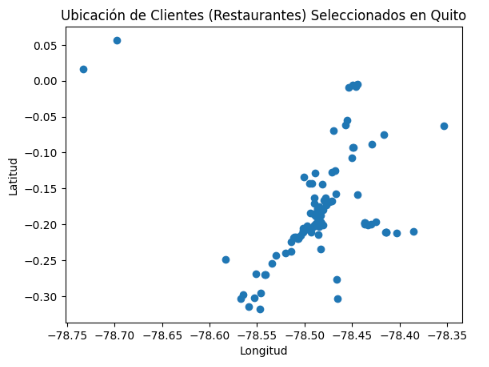
\includegraphics[width=0.7\linewidth]{ubicaciones.png}
    \caption{Muestra de 100 ubicaciones aleatorias}
    \label{fig:enter-label}
\end{figure}

\begin{figure}[h!]
    \centering
    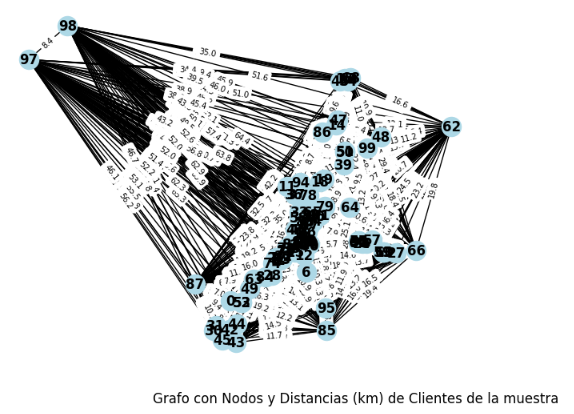
\includegraphics[width=0.6\linewidth]{grafoinicial.png}
    \caption{Grafo generado con las 100 muestras}
    \label{fig:enter-label}
\end{figure}




\section{Distribución de Rutas en los Camiones con k-means}

Para abordar el problema de múltiples camiones, utilizamos el algoritmo de k-means para dividir el conjunto de clientes en k grupos, donde k es el número de camiones disponibles. El proceso es el siguiente:
\begin{itemize}
    \item Agrupamiento Inicial: Aplicamos k-means para agrupar los clientes en 15 clusters, cada uno correspondiente a un camión.
    \item Asignación de Clientes a Camiones: Los clientes en cada cluster se asignan al camión correspondiente.
    \item Optimización de Rutas: Dentro de cada cluster, optimizamos la ruta usando los algoritmos mencionados (Greedy, Simulated Annealing, Quantum Annealing, QAOA, y Quantum Walks) y aplicamos 2-opt para refinar las rutas y reducir la distancia total recorrida.
\end{itemize}

Este enfoque permite una distribución inicial equilibrada de los clientes entre los camiones, mejorando así la eficiencia en la planificación y ejecución de las rutas de entrega.

\textbf{Pseudocódigo:}

\begin{tcolorbox}[colback=white!95!blue, colframe=blue!50!black, title=Kmeans, fontupper=\ttfamily]
\begin{enumerate}
    \item Aplicar K-means para agrupar clientes en `num\_camiones` clústeres.
    \item Para cada camión:
    \begin{itemize}
        \item Inicializar ruta con el depósito y los clientes del clúster.
        \item Utilizar paseos cuánticos para explorar el espacio de soluciones y encontrar una ruta inicial.
        \item Aplicar algoritmo 2-opt para optimizar la ruta.
    \end{itemize}
    \item Calcular la distancia total recorrida por todos los camiones.
\end{enumerate}
\end{tcolorbox}

\section{Implementación de Algoritmos Clásicos}

\subsection{Algoritmo 2-opt}

El algoritmo 2-opt es una técnica de optimización local utilizada para mejorar soluciones de problemas de optimización combinatoria. En nuestro caso, hemos adaptado el algoritmo 2-opt para refinar las rutas generadas por todos los algoritmos de optimización siguiendo estos pasos:
\begin{itemize}
	\item Inicialización: Comenzamos con una ruta generada por uno de los algoritmos principales (Greedy, Simulated Annealing, Quantum Annealing, QAOA, Quantum Walks).
    \item Iteración: Iteramos sobre cada par de aristas en la ruta actual y consideramos el intercambio de sus extremos para ver si la nueva ruta resultante es más corta.
    \item Intercambio de Aristas: Si encontramos un par de aristas cuyo intercambio resulta en una ruta más corta, realizamos el intercambio.
    \item Repetición: Repetimos este proceso hasta que no se puedan encontrar más mejoras en la ruta.
Este método permite mejorar iterativamente la calidad de las soluciones iniciales proporcionadas por los algoritmos principales, asegurando que las rutas finales sean lo más cortas posible.
\end{itemize}

\begin{tcolorbox}[colback=white!95!blue, colframe=blue!50!black, title=Algoritmo 2-opt, fontupper=\ttfamily]
	\begin{enumerate}
		\item Inicializar la mejor ruta del algoritmo principal
		\item Repetir
		\begin{itemize}
			\item Establecer mejorado como Falso
			\item Para i desde 1 hasta longitud(ruta) - 2 hacer
			\begin{itemize}
				\item Para j desde i + 1 hasta longitud(ruta) hacer
				\begin{itemize}
					\item Si j - i == 1 continuar
					\item Generar una nueva ruta intercambiando las aristas (i, i+1) y (j, j+1)
					\item Si la nueva ruta es más corta que la mejor ruta
						\item Actualizar la mejor ruta a la nueva ruta hasta que no mejore.
				\end{itemize}
			\end{itemize}    
			\item Devolver la mejor ruta
		\end{itemize}
	\end{enumerate}
\end{tcolorbox}


\subsection{Algoritmo Greedy}

Para adaptar el algoritmo Greedy a nuestro problema, comenzamos en el nodo de inicio (el depósito) y seleccionamos iterativamente el nodo más cercano no visitado hasta que todos los nodos hayan sido visitados. Finalmente, volvemos al nodo de inicio para completar la ruta. Este enfoque es simple pero puede resultar en soluciones subóptimas.

\textbf{Pseudocódigo:}
\begin{tcolorbox}[colback=white!95!blue, colframe=blue!50!black, title=Algoritmo Greedy, fontupper=\ttfamily]
\begin{enumerate}
    \item Iniciar en un nodo aleatorio.
    \item Mientras no se hayan visitado todos los nodos hacer:
    \begin{enumerate}
        \item Seleccionar el nodo más cercano no visitado.
        \item Añadir el nodo seleccionado a la ruta.
        \item Marcar el nodo seleccionado como visitado.
    \end{enumerate}
    \item Añadir el nodo inicial al final de la ruta para completar el ciclo.
    \item Devolver la ruta
\end{enumerate}
\end{tcolorbox}


\subsection{Algoritmo Simulated Annealing}

Para adaptar Simulated Annealing a nuestro problema, inicialmente generamos una solución aleatoria y evaluamos su longitud. Luego, iterativamente generamos nuevas soluciones mediante permutaciones aleatorias de la ruta actual y las evaluamos. Aceptamos nuevas soluciones basadas en un criterio de probabilidad que disminuye con el tiempo (temperatura). Este proceso permite escapar de óptimos locales y encontrar soluciones cercanas al óptimo global.


\begin{tcolorbox}[colback=white!95!blue, colframe=blue!50!black, title=Algoritmo de Recocido Simulado (SA), fontupper=\ttfamily]
\begin{enumerate}
    \item Inicializar la temperatura y la solución actual.
    \item Mientras la temperatura no sea mínima:
    \begin{enumerate}
        \item Generar una solución vecina.
        \item Evaluar el cambio en la calidad de la solución.
        \item Aceptar o rechazar la nueva solución basada en la probabilidad de aceptación.
        \item Reducir la temperatura.
    \end{enumerate}
    \item Retornar la mejor solución encontrada.
\end{enumerate}
\end{tcolorbox}



\section{Implementación de Algoritmos Cuánticos}

\subsection{Algoritmo Quantum Annealing}

En nuestro problema, Quantum Annealing se usa para resolver la formulación QUBO del TSP. Inicializamos el sistema cuántico en el estado fundamental de un Hamiltoniano simple y lo evolucionamos adiabáticamente hacia el Hamiltoniano del problema. La medición del estado final del sistema nos da la ruta óptima.

\textbf{Pseudocódigo:}
\begin{tcolorbox}[colback=white!95!blue, colframe=blue!50!black, title=Quantum Annealing (QA), fontupper=\ttfamily]
\begin{enumerate}
    \item Definir el problema en términos de QUBO.
    \item Preparar el sistema en el estado fundamental de \(H_0\).
    \item Evolucionar el sistema hacia \(H_1\) de manera adiabática.
    \item Medir el estado final para obtener la solución óptima.
\end{enumerate}
\end{tcolorbox}

\subsection{Algoritmo QAOA}

Para QAOA, preparamos un estado inicial de superposición uniforme y aplicamos secuencialmente operadores unitarios parametrizados que dependen de un Hamiltoniano de mezclado y el Hamiltoniano del problema. Usamos un algoritmo clásico para optimizar los parámetros de estos operadores, y la medición del estado final proporciona la ruta aproximada.


\textbf{Pseudocódigo:}
\begin{tcolorbox}[colback=white!95!blue, colframe=blue!50!black, title=Quantum Approximate Optimization Algorithm (QAOA), fontupper=\ttfamily]
\begin{enumerate}
    \item Preparar el estado inicial en superposición.
    \item Aplicar operadores \(U(H_B, \gamma)\) y \(U(H_C, \beta)\) secuencialmente.
    \item Optimizar \(\gamma\) y \(\beta\) mediante un algoritmo clásico.
    \item Medir el estado final para obtener la solución aproximada.
\end{enumerate}
\end{tcolorbox}


\subsection{Algoritmo Quantum Walks}
En el caso de Quantum Walks, inicializamos el estado cuántico del sistema y aplicamos un operador de evolución repetidamente. Este enfoque permite explorar el espacio de soluciones de manera eficiente. La medición del estado final nos da la ruta óptima.

\begin{tcolorbox}[colback=white!95!blue, colframe=blue!50!black, title=Quantum Walks (QW), fontupper=\ttfamily]
\begin{enumerate}
    \item Inicializar el estado cuántico del sistema.
    \item Definir las operaciones de moneda y shift.
    \item Aplicar repetidamente las operaciones de moneda y shift.
    \item Medir el estado final para obtener la solución óptima.
\end{enumerate}
\end{tcolorbox}


\chapter{Resultados y Análisis}

En este capítulo, se presentan y analizan los resultados obtenidos al aplicar tanto algoritmos clásicos como cuánticos para la optimización de rutas analizados. Los algoritmos evaluados incluyen Greedy, Recocido Simulado (Simulated Annealing), Quantum Annealing, Quantum Approximate Optimization Algorithm (QAOA) y Quantum Walks. Además, se ha utilizado el algoritmo de k-means para distribuir las rutas entre los camiones y el algoritmo 2-opt para optimizar localmente las soluciones generadas.

\section{Metodología de Evaluación}

\subsection{Métricas de Evaluación}

Las métricas principales utilizadas para la evaluación de los algoritmos fueron:

\begin{itemize}
    \item \textbf{Distancia Total Recorrida (km):} La suma de las distancias recorridas por todos los camiones en sus rutas de entrega.
    \item \textbf{Tiempo de Ejecución del Algoritmo (ms):} El tiempo necesario para que el algoritmo genere una solución.
    \item \textbf{Tiempo de Ejecución del Código (s):} El tiempo total que incluye la ejecución del código en las plataformas cuánticas y clásicas unto con las metricas y graficos generados dentr del codigo.
\end{itemize}

\subsection{Configuración Experimental}

Para realizar la evaluación, se generaron muestras de 100 clientes con ubicaciones aleatorias. Las distancias entre los clientes se calcularon utilizando la distancia Manhattan. Los algoritmos se ejecutaron en un entorno controlado para asegurar la comparabilidad de los resultados.

\section{Resultados Obtenidos}

\subsection{Comparación General de Algoritmos}

La Tabla \ref{tab:comparison} muestra una comparación de los resultados obtenidos para cada algoritmo evaluado. Los algoritmos cuánticos (Quantum Annealing, QAOA y Quantum Walks) se evaluaron en la plataforma cuánticas D-Wave, mientras que los algoritmos clásicos (Greedy y Simulated Annealing) se ejecutaron en una computadora convencional.

\begin{table}[H]
\centering
\begin{tabular}{|m{5cm}|m{3cm}|m{3cm}|m{3cm}|}
\hline
\textbf{Algoritmo} & \textbf{Distancia} & \multicolumn{2}{c|}{\textbf{Tiempos de ejecución}} \\ \cline{3-4}
& \textbf{(km)} & \textbf{Algoritmo (ms)} & \textbf{Código (s)} \\ \hline
Greedy & 766,73 & 258,6 & 107 \\ \hline
Simulated Annealing & 765,24 & 315,8 & 45 \\ \hline
Quantum Annealing & 767,83 & 55,5 & 83,88 \\ \hline
QAOA & 767,83 & 52,4 & 81,8 \\ \hline
Quantum Walks & 767,83 & 48,5 & 76,3 \\ \hline
\end{tabular}
\caption{Comparación de Algoritmos}
\label{tab:comparison}
\end{table}

\subsection{Análisis de Distancias Recorridas}

Los resultados indican que el algoritmo de Recocido Simulado (Simulated Annealing) logró la menor distancia total recorrida (765,24 km), seguido de cerca por el algoritmo Greedy (766,73 km). Los algoritmos cuánticos mostraron distancias recorridas similares (767,83 km), lo cual demuestra su capacidad para generar soluciones competitivas.

\subsection{Análisis de Tiempos de Ejecución}

En términos de tiempos de ejecución del algoritmo, los algoritmos cuánticos fueron significativamente más rápidos que los clásicos. Quantum Walks tuvo el menor tiempo de ejecución del algoritmo (48,5 ms), seguido de QAOA (52,4 ms) y Quantum Annealing (55,5 ms). Esto resalta la eficiencia computacional de los algoritmos cuánticos en comparación con sus contrapartes clásicas.

\subsection{Análisis de Eficiencia en la Computación Cuántica}

Aunque los algoritmos cuánticos demostraron ser más rápidos en la ejecución del algoritmo, el tiempo total de ejecución del código fue mayor debido a la interacción con las plataformas cuánticas. Este tiempo adicional incluye la latencia de comunicación con el hardware cuántico y la inicialización del sistema.

\section{Visualización de Resultados}

\subsection{Solución Óptima Clásica}

La Figura \ref{fig:solucionSA2opt} muestra las rutas generadas por el algoritmo de Recocido Simulado optimizado con 2-opt y k-means.

\begin{figure}[H]
\centering
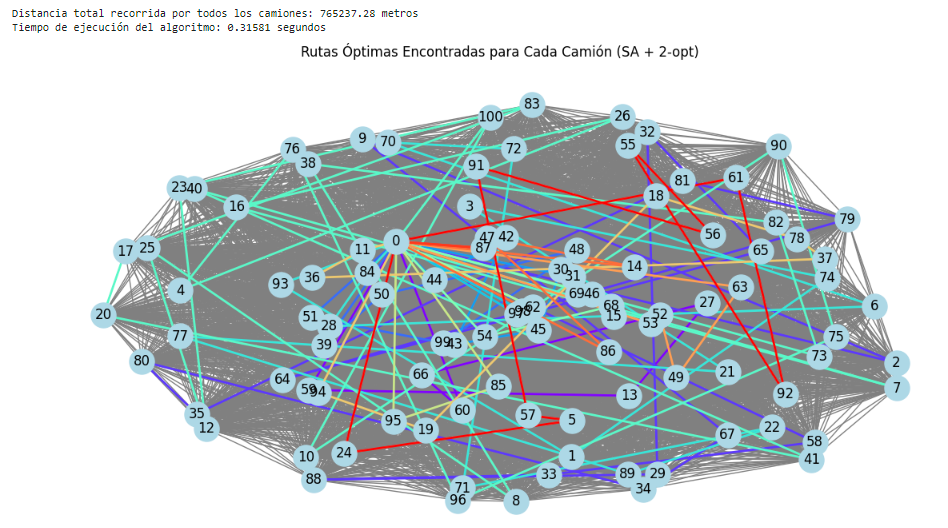
\includegraphics[width=1\linewidth]{solucionSA2opt.png}
\caption{Rutas con Simulated Annealing optimizado con 2-opt y k-means}
\label{fig:solucionSA2opt}
\end{figure}

\subsection{Solución Óptima Cuántica}

La Figura \ref{fig:solucionQW2opt} muestra las rutas generadas por el algoritmo Quantum Walks optimizado con 2-opt y k-means.

\begin{figure}[H]
\centering
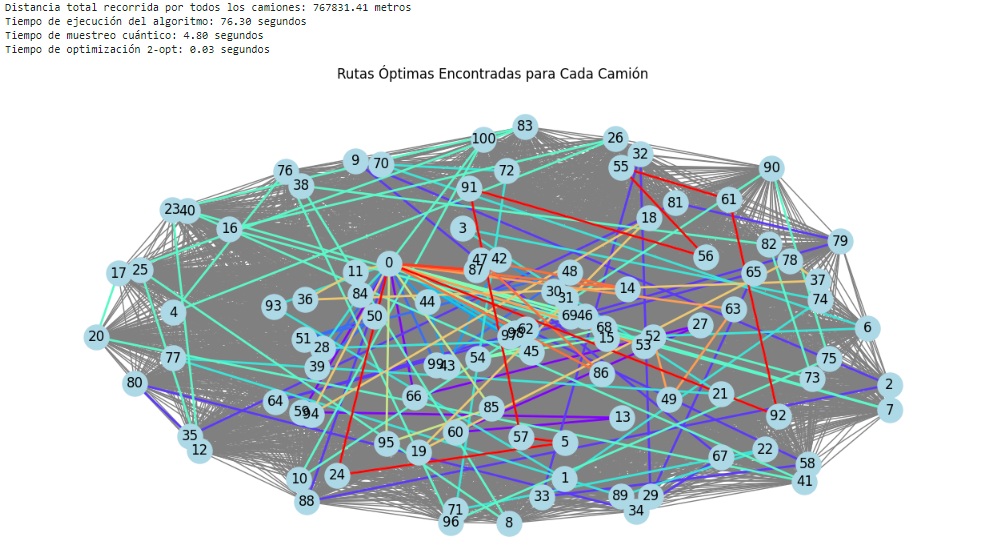
\includegraphics[width=1.1\linewidth]{solucionQW2opt.png}
\caption{Rutas con Quantum Walks optimizado con 2-opt y k-means}
\label{fig:solucionQW2opt}
\end{figure}

\section{Conclusiones}

\subsection{Rendimiento de los Algoritmos Cuánticos}

Los algoritmos cuánticos demostraron ser eficientes en términos de tiempo de ejecución del algoritmo, logrando tiempos significativamente menores que los algoritmos clásicos. Sin embargo, la distancia total recorrida fue ligeramente mayor en comparación con los mejores algoritmos clásicos, lo que sugiere que los algoritmos cuánticos aún tienen margen de mejora en términos de optimización de rutas.

\subsection{Viabilidad Técnica y Económica}

La implementación de soluciones cuánticas en la logística de transporte es técnicamente viable y muestra una promesa significativa en términos de eficiencia computacional. No obstante, la latencia de comunicación con el hardware cuántico y los costos asociados a su uso deben considerarse cuidadosamente para evaluar la viabilidad económica.

\subsection{Recomendaciones para Futuros Trabajos}

Se recomienda continuar explorando y refinando los algoritmos cuánticos para mejorar su rendimiento en términos de distancia recorrida. Además, es importante investigar formas de reducir la latencia de comunicación con el hardware cuántico y optimizar los tiempos de ejecución del código. La integración de algoritmos cuánticos con técnicas de aprendizaje automático podría ofrecer mejoras adicionales en la optimización de rutas y carga en el contexto de la logística de transporte.




\chapter{Conclusiones y Trabajo Futuro}

\section{Conclusiones}

El presente estudio abordó el desarrollo y aplicación de algoritmos cuánticos para la optimización de rutas de entrega y carga en la empresa Wolf, comparándolos con métodos clásicos. A continuación, se detallan las conclusiones principales obtenidas a partir de los resultados presentados en los capítulos anteriores.

\subsection{Rendimiento de Algoritmos Clásicos y Cuánticos}

Los resultados mostraron que los algoritmos cuánticos pueden ofrecer tiempos de ejecución significativamente menores en comparación con los algoritmos clásicos. En particular, el algoritmo Quantum Walks demostró ser el más eficiente en términos de tiempo de ejecución del algoritmo (48,5 ms), seguido de cerca por QAOA (52,4 ms) y Quantum Annealing (55,5 ms). Estos tiempos son considerablemente menores que los obtenidos por los algoritmos clásicos Greedy y Simulated Annealing, que registraron 258,6 ms y 315,8 ms respectivamente (ver Tabla \ref{tab:comparison}).

\subsection{Eficiencia en la Distancia Recorrida}

En términos de distancia total recorrida, los algoritmos clásicos mostraron un mejor rendimiento. El Recocido Simulado (Simulated Annealing) logró la menor distancia total recorrida (765,24 km), seguido por el algoritmo Greedy (766,73 km). Los algoritmos cuánticos presentaron distancias recorridas similares (767,83 km), lo que indica que aún hay margen de mejora para estos algoritmos en términos de optimización de rutas.

\subsection{Viabilidad Técnica y Económica}

La implementación de soluciones cuánticas en la logística de transporte es técnicamente viable y muestra una promesa significativa en términos de eficiencia computacional. Sin embargo, la latencia de comunicación con el hardware cuántico y los costos asociados a su uso deben considerarse cuidadosamente. Los tiempos de ejecución del código total, que incluyen la interacción con las plataformas cuánticas, fueron mayores para los algoritmos cuánticos en comparación con los clásicos. Esto sugiere la necesidad de optimizar las interfaces y la infraestructura de comunicación para aprovechar plenamente las ventajas de la computación cuántica.

\subsection{Impacto en la Logística de Transporte}

Los algoritmos cuánticos demostraron ser herramientas prometedoras para mejorar la eficiencia en la logística de transporte. La reducción en los tiempos de ejecución del algoritmo puede traducirse en una capacidad para procesar y optimizar rutas en tiempo real, lo cual es crucial en contextos de alta demanda y variabilidad. A pesar de que la distancia recorrida no fue óptima en comparación con los mejores algoritmos clásicos, la eficiencia computacional de los algoritmos cuánticos abre nuevas posibilidades para la optimización de rutas en tiempo real y a gran escala.

\section{Trabajo Futuro}

A partir de los resultados obtenidos, se identifican varias áreas de investigación futura que pueden contribuir a mejorar y expandir el uso de algoritmos cuánticos en la optimización de rutas y carga en logística.

\subsection{Mejora de Algoritmos Cuánticos}

Aunque los algoritmos cuánticos mostraron una gran eficiencia en términos de tiempo de ejecución, su rendimiento en términos de distancia recorrida puede ser mejorado. Futuros trabajos deberían enfocarse en:

\begin{itemize}
    \item \textbf{Optimización de Parámetros:} Investigar técnicas avanzadas de optimización de parámetros para algoritmos como QAOA y Quantum Annealing para mejorar su capacidad de encontrar soluciones más óptimas.
    \item \textbf{Híbridos Cuántico-Clásicos:} Desarrollar y evaluar algoritmos híbridos que combinen la eficiencia computacional de los métodos cuánticos con la precisión de los métodos clásicos, optimizando ambos aspectos.
    \item \textbf{Refinamiento de Heurísticas Cuánticas:} Implementar y probar nuevas heurísticas cuánticas que puedan reducir aún más las distancias recorridas sin sacrificar la eficiencia en tiempo.
\end{itemize}

\subsection{Reducción de Latencia y Costos de Computación Cuántica}

El tiempo adicional necesario para la comunicación con plataformas cuánticas es un área crítica a abordar. Se recomienda:

\begin{itemize}
    \item \textbf{Optimización de Infraestructura:} Investigar mejoras en la infraestructura de comunicación entre sistemas clásicos y cuánticos para reducir la latencia.
    \item \textbf{Economías de Escala:} Evaluar el impacto de las economías de escala en los costos de operación cuántica a medida que las tecnologías cuánticas se vuelvan más accesibles y asequibles.
\end{itemize}

\subsection{Aplicaciones en Tiempo Real y Escenarios Dinámicos}

La capacidad de los algoritmos cuánticos para procesar datos rápidamente los hace ideales para aplicaciones en tiempo real. Futuros trabajos pueden explorar:

\begin{itemize}
    \item \textbf{Implementación en Tiempo Real:} Desarrollar sistemas de optimización de rutas que utilicen algoritmos cuánticos para ajustar dinámicamente las rutas en función de datos en tiempo real, como el tráfico y las condiciones climáticas.
    \item \textbf{Escenarios Dinámicos:} Investigar cómo los algoritmos cuánticos pueden manejar cambios dinámicos en las rutas y carga, como cancelaciones de última hora o adiciones de nuevos destinos.
\end{itemize}

\subsection{Integración con Aprendizaje Automático}

La integración de algoritmos cuánticos con técnicas de aprendizaje automático puede ofrecer mejoras adicionales en la optimización de rutas y carga. Se sugiere:

\begin{itemize}
    \item \textbf{Modelos Predictivos:} Utilizar modelos de aprendizaje automático para predecir patrones de demanda y optimizar proactivamente las rutas utilizando algoritmos cuánticos.
    \item \textbf{Aprendizaje Reforzado:} Investigar el uso de algoritmos de aprendizaje reforzado cuántico para mejorar continuamente las rutas basadas en retroalimentación y datos históricos.
\end{itemize}

\section{Reflexión Final}

El trabajo realizado demuestra el potencial de la computación cuántica para transformar la optimización de rutas y la logística en general. A medida que las tecnologías cuánticas continúan avanzando, es probable que veamos una adopción más amplia y una mayor integración de estas técnicas en la industria. El camino hacia la optimización cuántica está lleno de oportunidades y desafíos, y el trabajo futuro será crucial para desbloquear todo su potencial.


\begin{thebibliography}{a}

	\bibitem[Nielsen(2010)]{nielsenChuang} \textsc{Nielsen, M. A. \& Chuang, I. L.} (2010),
	\textit{Quantum Computation and Quantum Information.}
	Cambridge University Press.
	
	\bibitem[QWalk(2021)]{QWalk-Based} \textsc{Bennett, T. and Matwiejew, E. and Marsh, S. and Wang, J. B.} (2021),
	\textit{Quantum Walk-Based Vehicle Routing Optimisation.}
	Frontiers in Physics.
	
	\bibitem[Farhi(2014)]{farhiQuantum} \textsc{Farhi, E., Goldstone, J., \& Gutmann, S.} (2014),
	\textit{A Quantum Approximate Optimization Algorithm.}
	arXiv:1411.4028.
	
	\bibitem[Grover(1997)]{groverAlgorithm} \textsc{Grover, L. K.} (1997),
	\textit{Quantum Mechanics helps in searching for a needle in a haystack.}
	Physical Review Letters, 79(2), 325.
	
	\bibitem[Venegas(2003)]{quantumTransportOpt} \textsc{Venegas-Andraca, S. E., \& Bose, S.} (2003),
	\textit{Quantum Walk Algorithms for Transportation Networks.}
	Quantum Information \& Computation, 3(6), 563-574.
	
	\bibitem[Bertsimas(1996)]{transportationScience} \textsc{Bertsimas, D., \& Simchi-Levi, D.} (1996),
	\textit{A New Generation of Vehicle Routing Research: Robust Algorithms, Addressing Uncertainty.}
	Operations Research, 44(2), 286-304.
	
	\bibitem[Gibney(2019)]{quantumTech} \textsc{Gibney, E.} (2019),
	\textit{Quantum gold rush: the private funding pouring into quantum start-ups.}
	Nature, 574, 22-24.
	
	\bibitem[Abraham(2019)]{qiskit} \textsc{Abraham, H., et al.} (2019),
	\textit{Qiskit: An Open-source Framework for Quantum Computing.}
	Accessed via https://qiskit.org.
	
	\bibitem[Dwave(2020)]{dwaveOcean} \textsc{D-Wave Systems Inc.} (2020),
	\textit{Ocean Software Documentation.}
	Accessed via https://docs.ocean.dwavesys.com/en/latest.
	
		
	\bibitem[Shor(1994)]{shorAlgorithm} \textsc{Shor, P. W.} (1994),
	\textit{Algorithms for Quantum Computation: Discrete Logarithms and Factoring.}
	Proceedings 35th Annual Symposium on Foundations of Computer Science.
	
	\bibitem[Farhi et al.(2014)]{farhiQuantum} \textsc{Farhi, E., Goldstone, J., \& Gutmann, S.} (2014),
	\textit{A Quantum Approximate Optimization Algorithm.}
	arXiv:1411.4028.
	
	\bibitem[Gibney(2019)]{gibneyQuantumTech} \textsc{Gibney, E.} (2019),
	\textit{Quantum gold rush: the private funding pouring into quantum start-ups.}
	Nature, 574, 22-24.

	\bibitem[Clarke y Wright(1964)]{clarkeWright} \textsc{Clarke, G. \& Wright, J. W.} (1964),
	\textit{Scheduling of Vehicles from a Central Depot to a Number of Delivery Points.}
	Operations Research, 12(4), 568-581.
	
	\bibitem[Glover(1989)]{glover1989tabu} \textsc{Glover, F.} (1989),
	\textit{Tabu Search—Part I.}
	ORSA Journal on Computing, 1(3), 190-206.
	
	\bibitem[Dorigo et al.(1997)]{dorigo1997ant} \textsc{Dorigo, M., Maniezzo, V., \& Colorni, A.} (1997),
	\textit{Ant System: Optimization by a Colony of Cooperating Agents.}
	IEEE Transactions on Systems, Man, and Cybernetics, Part B (Cybernetics), 26(1), 29-41.
	
	\bibitem[Kennedy y Eberhart(1995)]{kennedy1995particle} \textsc{Kennedy, J., \& Eberhart, R.} (1995),
	\textit{Particle Swarm Optimization.}
	Proceedings of ICNN'95 - International Conference on Neural Networks, 4, 1942-1948.
	
	\bibitem[Nemhauser y Wolsey(1999)]{nemhauser1999integer} \textsc{Nemhauser, G. L., \& Wolsey, L. A.} (1999),
	\textit{Integer and Combinatorial Optimization.} John Wiley \& Sons.
	
	\bibitem[Kirkpatrick et al.(1983)]{kirkpatrick1983optimization} \textsc{Kirkpatrick, S., Gelatt, C. D., \& Vecchi, M. P.} (1983),
	\textit{Optimization by Simulated Annealing.}
	Science, 220(4598), 671-680.
	
	\bibitem[Mladenović y Hansen(1997)]{mladenovic1997variable} \textsc{Mladenović, N., \& Hansen, P.} (1997),
	\textit{Variable Neighborhood Search.}
	Computers \& Operations Research, 24(11), 1097-1100.
	
	\bibitem[Holland(1992)]{holland1992adaptation} \textsc{Holland, J. H.} (1992),
	\textit{Adaptation in Natural and Artificial Systems.}
	MIT Press.
	
	\bibitem[Lawler(1985)]{lawler1985knapsack} \textsc{Lawler, E. L.} (1985),
	\textit{Knapsack Problems: Algorithms and Computer Implementations.}
	Wiley-Interscience Series in Discrete Mathematics and Optimization.
	
	\bibitem[Lawler y Wood(1966)]{lawler1966branch} \textsc{Lawler, E. L., \& Wood, D. E.} (1966),
	\textit{Branch-and-Bound Methods: A Survey.}
	Operations Research, 14(4), 699-719.
	
	\bibitem[Coffman et al.(1978)]{coffman1978application} \textsc{Coffman, E. G., Garey, M. R., Johnson, D. S.} (1978),
	\textit{An Application of Bin-Packing to Multiprocessor Scheduling.}
	SIAM Journal on Computing, 7(1), 1-17.
	
	\bibitem[Bellman(1966)]{bellman1966dynamic} \textsc{Bellman, R.} (1966),
	\textit{Dynamic Programming.}
	Science, 153(3731), 34-37.
	
	\bibitem[Johnson(1954)]{johnson1954optimal} \textsc{Johnson, S. M.} (1954),
	\textit{Optimal Two- and Three-Stage Production Schedules with Setup Times Included.}
	Naval Research Logistics Quarterly, 1(1), 61-68.
	
	\bibitem[Rossi et al.(2006)]{rossi2006handbook} \textsc{Rossi, F., Van Beek, P., \& Walsh, T.} (2006),
	\textit{Handbook of Constraint Programming.}
	Elsevier.
	
	\bibitem[Graham(1966)]{graham1966bounds} \textsc{Graham, R. L.} (1966),
	\textit{Bounds on Multiprocessing Timing Anomalies.}
	SIAM Journal on Applied Mathematics, 17(2), 416-429.
	
	\bibitem[Phillipson(2024)]{phillipson2024} \textsc{Phillipson, F.} (2024),
	\textit{Quantum Computing in Logistics and Supply Chain Management - an Overview.}
	Maastricht University, arXiv:2402.17520.

    \bibitem[Cormen(2009)]{Cormen2009} 
    \textsc{Cormen, Thomas H. and Leiserson, Charles E. and Rivest, Ronald L. and Stein, Clifford} (2009),
	\textit{Introduction to Algorithms.}
	MIT Press. fourth edition.

    \bibitem[kempe(2003)]{kempe2003}
    \textsc{Kempe, Julia},
    \textit{Quantum random walks: an introductory overview},
    Taylor \& Francis, Contemporary Physics. 44.4 (2003): 307-327.

    \bibitem[childs(2002)]{childs2002}
    \textsc{Childs, Andrew M., Edward Farhi, and Sam Gutmann.}
    \textit{Example of the difference between quantum and classical random walks}.
    Quantum Information Processing, 1.1-2 (2002): 35-43.    

    \bibitem[lawler(1985)]{lawler1985}
    \textsc{Lawler, Eugene L., Lenstra, Jan Karel, Rinnooy Kan, Alexander Hendrik George, and Shmoys, David B.}
    \textit{The Traveling Salesman Problem: A Guided Tour of Combinatorial Optimization}. 
    John Wiley \& Sons, Inc., 1985.

\end{thebibliography}

\appendix

\chapter{Apendices}

\section{Codigo Algoritmo Greedy}

\lstset{frame=single}
\begin{lstlisting}
import random
import numpy as np
from sklearn.cluster import KMeans

# Initialization
nodes = initialize_nodes()
distances = calculate_distances(nodes)

# Apply k-means to cluster nodes into k clusters
k = number_of_clusters
kmeans = KMeans(n_clusters=k)
clusters = kmeans.fit_predict(nodes)

routes = []
for cluster in range(k):
    cluster_nodes = [node for i, node in enumerate(nodes) if clusters[i] == cluster]
    route = [starting_node]
    
    # Greedy Algorithm
    while cluster_nodes:
        current_node = route[-1]
        next_node = min(cluster_nodes, key=lambda node: distances[current_node][node])
        route.append(next_node)
        cluster_nodes.remove(next_node)
    routes.append(route)

# 2-opt Optimization
for route in routes:
    improvement = True
    while improvement:
        improvement = False
        for i in range(1, len(route) - 2):
            for j in range(i + 1, len(route)):
                if j - i == 1:
                    continue
                new_route = route[:i] + route[i:j][::-1] + route[j:]
                if calculate_route_distance(new_route, distances) < calculate_route_distance(route, distances):
                    route = new_route
                    improvement = True
\end{lstlisting}






\section{Codigo Algoritmo Simulated Annealing}

\begin{lstlisting}
import random
import numpy as np
from sklearn.cluster import KMeans

# Initialization
nodes = initialize_nodes()
distances = calculate_distances(nodes)

# Apply k-means to cluster nodes into k clusters
k = number_of_clusters
kmeans = KMeans(n_clusters=k)
clusters = kmeans.fit_predict(nodes)

routes = []
for cluster in range(k):
    cluster_nodes = [node for i, node in enumerate(nodes) if clusters[i] == cluster]
    route = initial_random_route(cluster_nodes)
    current_temp = initial_temp
    
    # Simulated Annealing Algorithm
    while current_temp > final_temp:
        new_route = generate_neighbor(route)
        delta = calculate_route_distance(new_route, distances) - calculate_route_distance(route, distances)
        if delta < 0 or random.random() < np.exp(-delta / current_temp):
            route = new_route
        current_temp = cool_down(current_temp)
    routes.append(route)

# 2-opt Optimization
for route in routes:
    improvement = True
    while improvement:
        improvement = False
        for i in range(1, len(route) - 2):
            for j in range(i + 1, len(route)):
                if j - i == 1:
                    continue
                new_route = route[:i] + route[i:j][::-1] + route[j:]
                if calculate_route_distance(new_route, distances) < calculate_route_distance(route, distances):
                    route = new_route
                    improvement = True
\end{lstlisting}





\section{Codigo Algoritmo Quantum Annealing}

\begin{lstlisting}
import random
import numpy as np
from sklearn.cluster import KMeans
from dwave.system import DWaveSampler, EmbeddingComposite
import dimod

# Initialization
nodes = initialize_nodes()
distances = calculate_distances(nodes)

# Apply k-means to cluster nodes into k clusters
k = number_of_clusters
kmeans = KMeans(n_clusters=k)
clusters = kmeans.fit_predict(nodes)

routes = []
for cluster in range(k):
    cluster_nodes = [node for i, node in enumerate(nodes) if clusters[i] == cluster]
    QUBO = construct_QUBO(cluster_nodes, distances)
    sampler = EmbeddingComposite(DWaveSampler())
    response = sampler.sample_qubo(QUBO)
    route = get_route_from_response(response)
    routes.append(route)

# 2-opt Optimization
for route in routes:
    improvement = True
    while improvement:
        improvement = False
        for i in range(1, len(route) - 2):
            for j in range(i + 1, len(route)):
                if j - i == 1:
                    continue
                new_route = route[:i] + route[i:j][::-1] + route[j:]
                if calculate_route_distance(new_route, distances) < calculate_route_distance(route, distances):
                    route = new_route
                    improvement = True
\end{lstlisting}


\section{Codigo Algoritmo QAOA}

\begin{lstlisting}
import random
import numpy as np
from sklearn.cluster import KMeans
from qiskit import Aer, execute
from qiskit.optimization.applications.ising import tsp
from qiskit.aqua.algorithms import QAOA
from qiskit.aqua.components.optimizers import COBYLA

# Initialization
nodes = initialize_nodes()
distances = calculate_distances(nodes)

# Apply k-means to cluster nodes into k clusters
k = number_of_clusters
kmeans = KMeans(n_clusters=k)
clusters = kmeans.fit_predict(nodes)

routes = []
for cluster in range(k):
    cluster_nodes = [node for i, node in enumerate(nodes) if clusters[i] == cluster]
    qubit_op, offset = tsp.get_operator(matrix)

    # QAOA parameters
    p = 1
    optimizer = COBYLA(maxiter=250)
    qaoa = QAOA(qubit_op, optimizer, p)
    backend = Aer.get_backend('statevector_simulator')
    result = qaoa.run(backend)
    route = tsp.sample_most_likely(result['eigvecs'][0])
    routes.append(route)

# 2-opt Optimization
for route in routes:
    improvement = True
    while improvement:
        improvement = False
        for i in range(1, len(route) - 2):
            for j in range(i + 1, len(route)):
                if j - i == 1:
                    continue
                new_route = route[:i] + route[i:j][::-1] + route[j:]
                if calculate_route_distance(new_route, distances) < calculate_route_distance(route, distances):
                    route = new_route
                    improvement = True
\end{lstlisting}



\section{Codigo Algoritmo Quantum Walks}

\begin{lstlisting}
import random
import numpy as np
from sklearn.cluster import KMeans
from dwave.system import DWaveSampler, EmbeddingComposite
import dimod

# Initialization
nodes = initialize_nodes()
distances = calculate_distances(nodes)

# Apply k-means to cluster nodes into k clusters
k = number_of_clusters
kmeans = KMeans(n_clusters=k)
clusters = kmeans.fit_predict(nodes)

routes = []
for cluster in range(k):
    cluster_nodes = [node for i, node in enumerate(nodes) if clusters[i] == cluster]
    QUBO = construct_QUBO(cluster_nodes, distances)
    sampler = EmbeddingComposite(DWaveSampler())
    response = sampler.sample_qubo(QUBO)
    route = get_route_from_response(response)
    routes.append(route)

# 2-opt Optimization
for route in routes:
    improvement = True
    while improvement:
        improvement = False
        for i in range(1, len(route) - 2):
            for j in range(i + 1, len(route)):
                if j - i == 1:
                    continue
                new_route = route[:i] + route[i:j][::-1] + route[j:]
                if calculate_route_distance(new_route, distances) < calculate_route_distance(route, distances):
                    route = new_route
                    improvement = True
\end{lstlisting}


\section{Mejor resultado de algortimos Clásico y Cuántico}

\begin{figure}[h!]
    \centering
    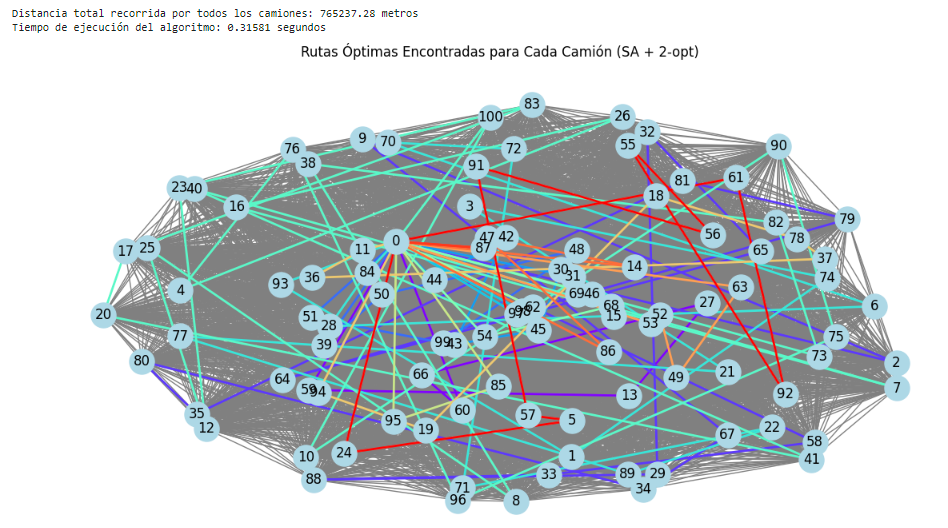
\includegraphics[width=1\linewidth]{solucionSA2opt.png}
    \caption{Rutas con SA optimizado con 2-opt y K-means}
    \label{fig:enter-label}
\end{figure}



\begin{figure}[h]
    \centering
    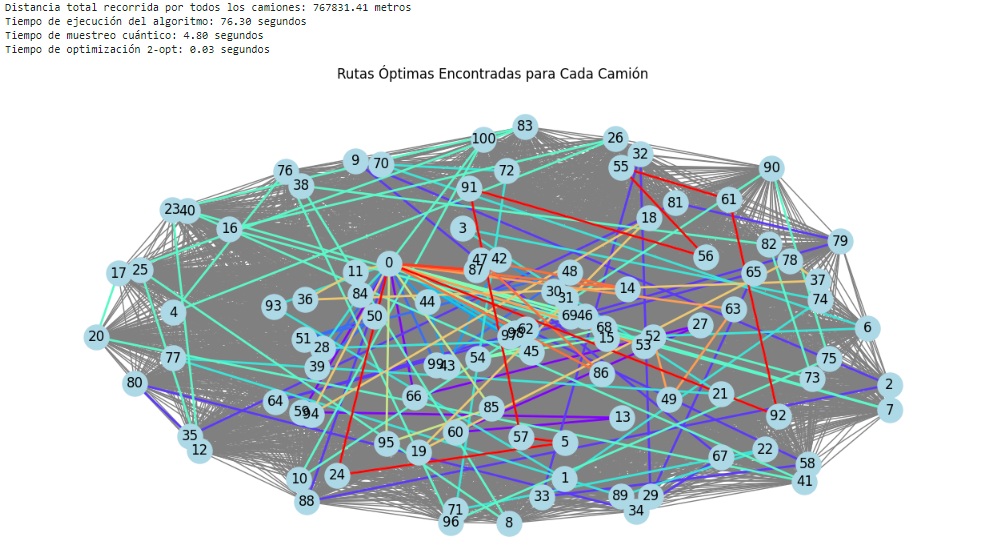
\includegraphics[width=1.1\linewidth]{solucionQW2opt.png}
    \caption{Rutas con QW optimizado con 2-opt y K-means}
    \label{fig:enter-label}
\end{figure}

\end{document}
